\documentclass[11pt, a4paper]{article}

\title{Dynamic Rate Control for Retro Game Emulators}
\author{Hans-Kristian Arntzen}

\usepackage{amsmath}
\usepackage{float}
\usepackage{graphicx}

\begin{document}
\maketitle

\begin{abstract}
This article describes a method for game emulator frontends
to synchronize both audio and video output at the same time, even
when the emulating system has a different refresh rate and audio sampling rate
than the gaming system that is being emulated.

The method works by dynamically adjusting audio resampling ratios in such ways that
ideally, the audio buffer is never underrun nor overrun, thus avoiding blocking on audio.
This in turn allows vertical synchronization for video.

The audio pitch is adjusted when adjusting audio resampling ratios,
but in practice so little, that it is inaudible to the human ear.
\end{abstract}

\section{Background}

Retro game consoles are highly synchronous. Their audio output rates are linked directly
to video refresh rates. Every video frame, the audio chip generates on average a fixed amount of audio samples. Before continuing to emulate the next frame, the generated audio samples must be pushed
to an audio buffer of fixed size.

If there is not enough space in the audio buffer, the emulator must wait (block) for the buffer to become ready for writing. This is a non-ideal situation as while the emulator is blocking on audio, a vertical refresh might be missed entirely, thus creating stuttering video.

\subsection{The ideal synchronization}
For an emulator of a retro game system, a key factor in smooth video is vertical refresh synchronization (VSync), where each frame of the game maps to a single frame on the monitor.
Audio must also be pushed to the speakers without any audio dropouts.
This double synchronization requirement poses a problem as any form of synchronization to one modality
will negatively affect the other.

This is a real problem as an emulator has no way of guaranteeing perfectly equal
video refresh rates and audio sampling rates as the original system.

On conventional computer hardware, there is no perfect way of knowing
the real monitor refresh rates and audio sampling rates either due to
tolerances on oscillators.

\subsection{Scope of method}
As this method aims to implement a method for synchronization when VSync is used,
this method is only useful when game frame rate is close to monitor frame rate.
If this is not the case, other methods should be employed.

\section{Method}
This method assumes that audio from the emulator is output at regular intervals, e.g.
every video frame. The method also assumes that audio is resampled from
the game system sampling rate to the sound cards sampling rate.
The resampling ratio will be dynamically adjusted every time audio is resampled and subsequently pushed to the audio buffer.

\subsection{Definitions}
\begin{itemize}
\item[$f_v$] Emulated game system frame rate (FPS)
\item[$f_a$] Emulated game system sampling rate (Hz)
\item[$r$] Emulated game system samples per frame $f_a / f_v$
\item[$m_a$] Emulator system sampling rate
\item[$m_v$] Emulator system monitor refresh rate
\item[$m_a^{'}$] Estimated emulator system sampling rate
\item[$m_v^{'}$] Estimated emulator system monitor refresh rate
\item[$R$] Emulator system samples per frame $m_a / m_v$
\item[$R^{'}$] Estimated emulator system samples per frame $m_a^{'} / m_v^{'}$
\item[$A_b$] Current amount of samples in the audio buffer
\item[$A_B$] Capacity (in samples) of the audio buffer
\item[$d$] Allowed deviation in audio pitch
\end{itemize}

\subsection{Resampling audio}
Every time the game system outputs audio, it is resampled with some ratio.
It is here assumed that the game system outputs a video frame worth of audio at a time.
While the formulae are invariant to how often audio is written to audio buffers, this assumption
is made for simplicity.

The correct resampling ratio is estimated to be $R^{'} / r$,
thus pushing $R^{'}$ samples of audio per frame on average.
In the duration of a frame, on average, $R$ audio frames will have been played to the speakers
and thus removed from the buffer.

\begin{equation}
\Delta A_b = R^{'} - R
\end{equation}

We see that unless $\Delta A_b = 0$, it is inevitable that the audio will either underrun ($A_b \leq 0$),
or block due to buffer being full ($A_b \geq A_B$).
Both these situations are not acceptable as underruns would cause audible audio dropouts,
and blocking would block the emulator from emulating more frames, and thus greatly increasing the chance of missing a VBlank, which is not acceptable as well. Blocking however, is far more preferable than underrunning.

As with any estimator, it is impossible to guarantee that $R^{'}$ can be perfectly estimated.
Therefore, it is impossible to guarantee that underrun nor blocking occurs.

\subsection{Dynamic rate control}
The proposed method will dynamically adjust the resampling ratio $R^{'} / r$.
Changing this ratio will adjust audio pitch as well. To ensure that these adjustments are not audible to the human ear, the range of adjustment will be limited by $d$.

Using $d$, the maximum pushed samples will be $R^{'} \left(1 + d\right)$,
and similarly, minimum will be $R^{'} \left(1 - d\right)$.
$d$ must be chosen so that $R$ falls between minimum or maximum. This depends on the confidence of the estimate $R^{'}$.

The revised update formula will look like this:

\begin{equation} \label{eq:update}
\Delta A_b = \left[ 1 + \left(\frac{A_B - 2A_b}{A_B}\right) d \right] R^{'} - R
\end{equation}

The formula will decrease resampling ratio if audio buffer is over half full, and similarly increase
resampling ratio if buffer is below half full.

\subsection{Stability}

To ensure that the method is stable, i.e. that $A_b$ will converge to a certain value,
we assume a continuous model for pushing audio.

\begin{equation}
\frac{\delta A_b}{\delta f} = \left[ 1 + \left(\frac{A_B - 2A_b}{A_B}\right) d \right] R^{'} - R
\end{equation}
\begin{equation} \label{eq:ab-diff}
\frac{\delta A_b}{\delta f} + \frac{2dR^{'}}{A_B}A_b = R^{'} \left(1 + d\right) - R
\end{equation}

The differential equation in \eqref{eq:ab-diff} can be solved as

\begin{equation}
A_b = A_B \frac{R^{'}\left(1 + d\right) - R}{2dR^{'}} + C_0\exp \left(-\frac{2dR^{'}}{A_B} f\right)
\end{equation}

Given time ($f \rightarrow \infty$), this expression converges to

\begin{equation}
A_{b,c} = A_B \frac{R^{'}\left(1 + d\right) - R}{2dR^{'}}
\end{equation}

If $R^{'}$ is the ideal estimate, $R^{'} = R$, the expression converges to

\begin{equation}
A_{b,c} = A_B / 2
\end{equation}
which is the best case, as having a half full buffer means most possible wiggle room for jitter.

\subsection{Updating ratio estimate $R^{'}$}
After time, it is assumed that $A_b$ will converge to $A_{b,c}$.
Due to jitter, and various non-ideal behavior, only an estimate of $A_{b,c}$, $\hat{A_{b,c}} = \bar{A_b}$ can be obtained.

\begin{equation}
\frac{\hat{R^{'}}}{R} = \frac{A_B}{\left(1 + d\right) A_B - 2d\hat{A_{b,c}}}
\end{equation}

The ratio estimate $R^{'}$ can thus be re-estimated accordingly. This method of re-estimating the ratio might however not be the best. Directly estimating $m_a^{'}$ and $m_v^{'}$ should yield more confident results, but this is outside the scope of this article.

\section{Results}

A synthetic test was carried out to test how the method would react to a common scenario for this method. An emulation of Super Nintendo Entertainment System (SNES) was matched to an emulating system.
To test effects of jitter, the frame time was assumed to follow a normal distribution.
Thus, $R$ in \eqref{eq:update} followed a normal distribution.

\begin{table}[H]
\centering
\caption{Timings}
\begin{tabular}{|c|c|c|}
	\hline
	System & FPS (Hz) & Sample rate (Hz)\\\hline
	SNES & 60.0988 & 32040.5\\\hline
	Emulating system & 59.88 & 48000.15\\\hline
	Estimated system & 59.95 & 48000.0\\\hline
\end{tabular}
\end{table}

\begin{table}[H]
\centering
\caption{Test parameters}
\begin{tabular}{|c|c|}
	\hline
	$d$ & $0.005$\\\hline
	Frame time deviation & $2 \%$\\\hline
\end{tabular}
\end{table}

\begin{figure}[H]
\centering
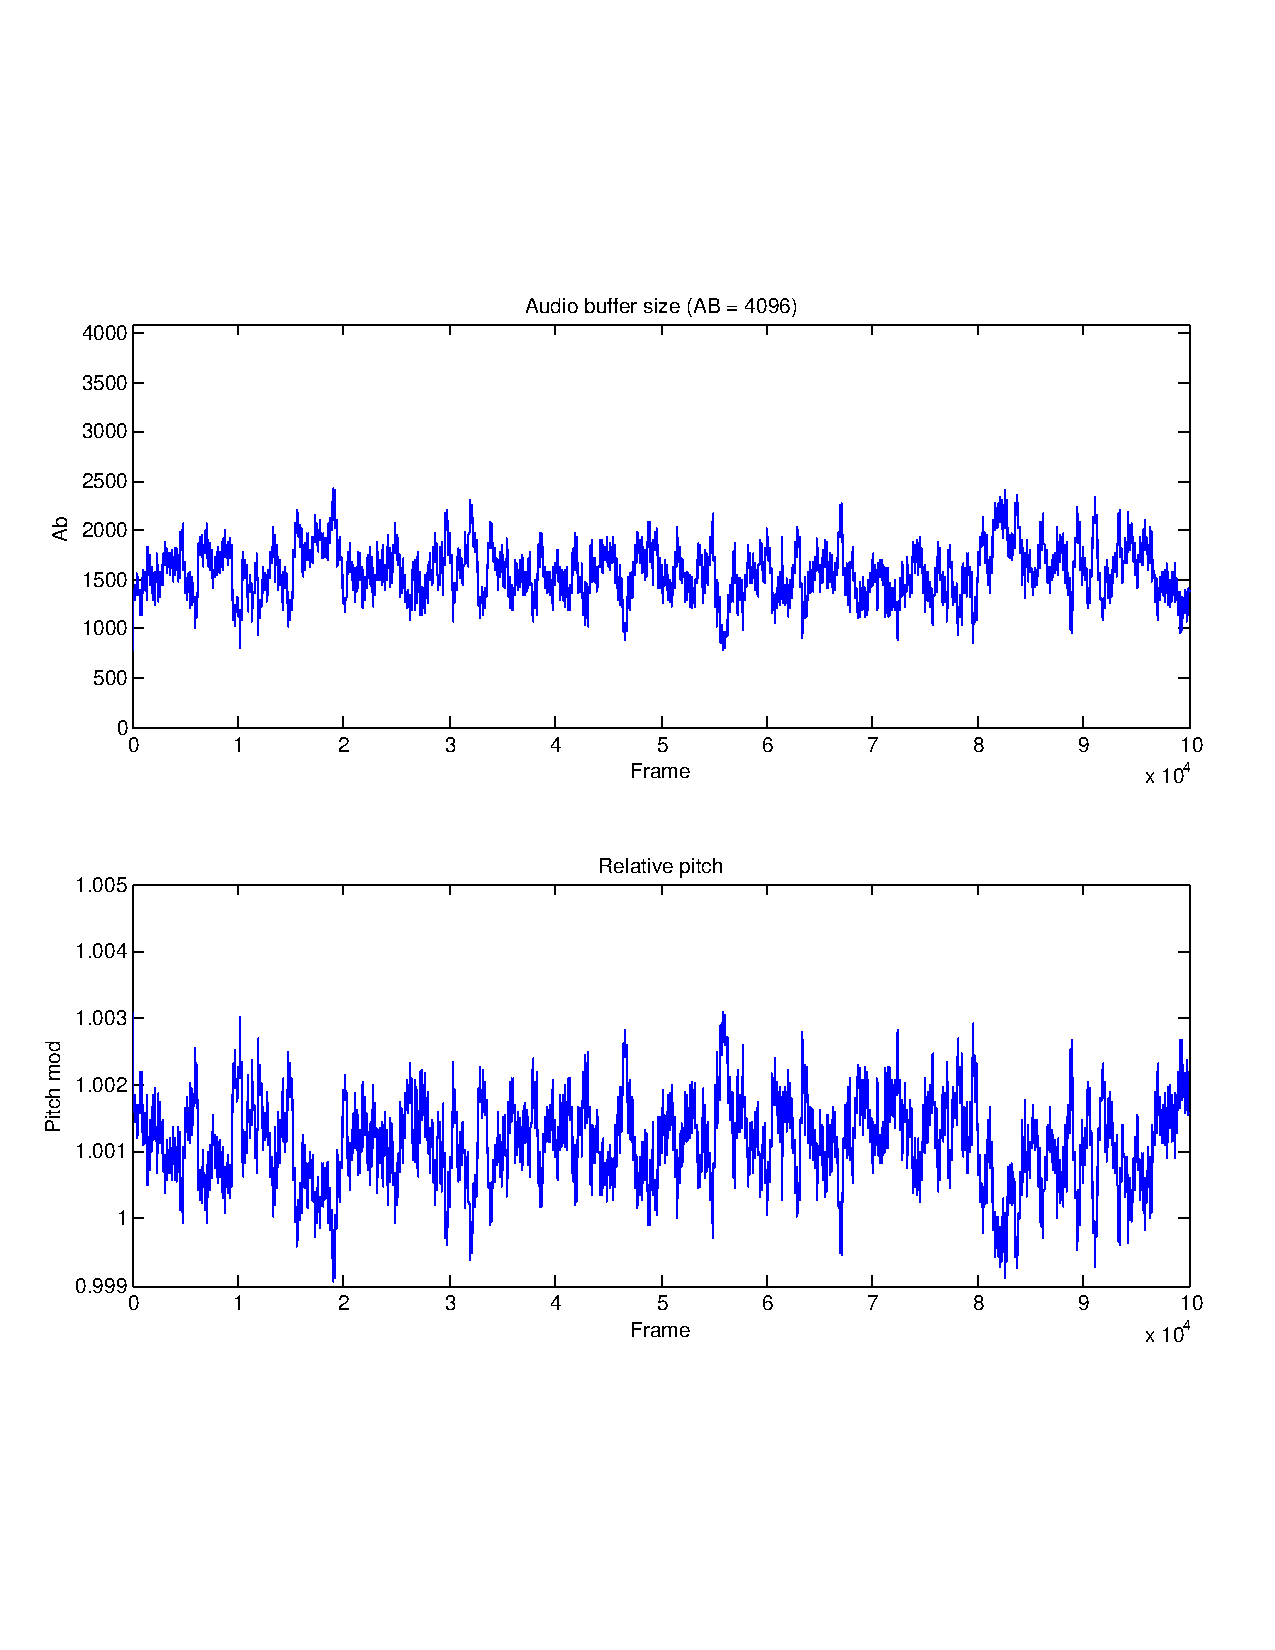
\includegraphics[width=12cm]{ratecontrol-data.pdf}
\caption{Results with 2\% standard deviation on frame time}
\end{figure}

The results are shown for audio buffer size over time and the pitch modulation for every simulated frame. Audio pitch modulation deviation was estimated to $0.062\%$, significantly lower than the $d$ value, which allowed for a maximum deviation of $0.5\%$.

The audio buffer is never filled nor underrun, which would allow every single VBlank to be met, while maintaining audio sync.

\section{Discussion}

\subsection{Effect of $d$}
Ideally, $d$ should be as low as possible to avoid large deviations in pitch, but at the same time, a too low value for $d$ will not be able to compensate for the difference between $R^{'}$ and $R$.
From testing in the emulator frontend RetroArch\footnote{https://github.com/Themaister/RetroArch}, a factor of $d \geq 0.002, d \leq 0.005$ has been found to give satisfactory results.

This method does not propose a method of determining the best $d$ factor.

\subsection{Audibility}
As audio pitch is altered, there is a question of audibility. Given a small enough $d$, it's
clear that the effect would be completely inaudible as all oscillators in a DAC have tolerances and jitter to some degree. It is also reasonable to believe that some persons are able to notice a smaller $d$ than others.

Some testing must be carried out to find a $d$ that is inaudible in subjective tests.

\section{Conclusion}
This method shows that it is possible to obtain synchronization to both VBlank and audio without having a perfect estimate of the emulating systems frequencies. As long as the estimates are reasonable close to the real values, the dynamic rate control method proposed here is able to smooth out the differences.

\end{document}